% Set up page specifications and import packages
\documentclass[11pt]{amsart}
\usepackage[margin=.5in]{geometry}          
\usepackage{graphicx}
\usepackage{amsthm, amsmath, amssymb}
\usepackage{setspace}
\setlength{\parindent}{0em}
\usepackage{epsfig,bm,color}
\usepackage{mathtools}

\DeclarePairedDelimiter{\ceil}{\lceil}{\rceil}

% Define commonly used commands with a shortcut
\newcommand{\Zpx}{\mathbb{Z}_p[x]}
\newcommand{\Z}{\mathbb{Z}}
\newcommand{\Q}{\mathbb{Q}}
\newcommand{\C}{\mathbb{C}}
\newcommand{\R}{\mathbb{R}}
\newcommand{\e}{\epsilon}
\newcommand{\adj}{\rightarrow}
\newcommand{\tab}{\hspace*{.75cm}}
\newcommand{\setTo}{\leftarrow}
\newcommand{\ul}{\underline}
\newcommand{\kap}{\kappa}

% Define document tittle and author
\title{MA4710 Project 5}
\author{Daniel Henderson}

% Begin document and make tittle
\begin{document}
\maketitle

{\bf\large Introduction}\\
This week we look at a variety of ways to detect collinearity between the numerical variables of my data set. The data set contains the same number of observations as last submission, though, a couple of the variables have been removed.
Specifically, height and weight are no longer present in the 'FullData.csv'.
This aids in keeping the code in model\_selection.R clean.
This is not a cause of major concern because body mass index is still a present column. 
However, there have been some uninvestigated interactions with these terms, which may add value to the model.\\

After investigating collinearity, we will determine a final model based upon on an exhaustive selection procedure.\\

\vspace{0.25in}
{\bf\large Collinearity Investigation on Full Model}\\
After parsing the "FullData.csv" file into a dataframe, we apply the following transformations:\\

\tab years\_climbing $\setTo$ ln(years\_climbing + 1)\\
\tab max\_pull $\setTo$ ln(max\_pull)\\
\tab max\_push $\setTo$ max\_push$^{-0.5}$ \\

These transformations address previously identified problems of our linearity assumption.
They where initially determined by an elegant rounding of the reported $\hat\lambda$ value from the invTransPlot function.
I determined that the condition number of the scaled covariance matrix of predictors to be $\kappa = 4.3$, which supports that claim that there are no significant signs of collinearity between our predictors.
For further evidence, consider the Variance Inflation Factors shown below\\

\begin{center}
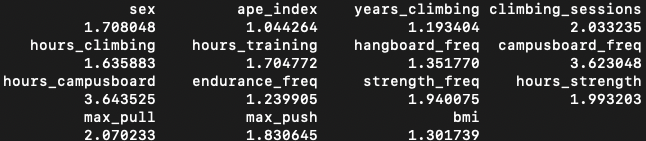
\includegraphics[width=0.7\textwidth]{vif}
\end{center}

Notice that campusboard\_freq and hours\_campusboard have the highest variance inflation factors.
Additionally, they are nearly identical.
This makes sense - there out to be relationship between the amount of times you engage in an exercise per week and the total number of hours doing the exercise per week.
The covariance between the two variables is $0.43$, which aligns with the above reasoning. 
However, both of these values are not a major concern according the crude rule of thumb that we should flag a VIF exceeding $10$.


\newpage
{\bf\large Variable Selection Proceduresl}\\
In the model\_selection.R script, we perform an exhaustive search over the columns of our dataframe to determine the "best" models of various size.
We let out intuition guide us and allow the sex variable to interacte pairwise with bmi as an option when we determine the best subset models.
Below are some diagnostic plots of this procedure:\\


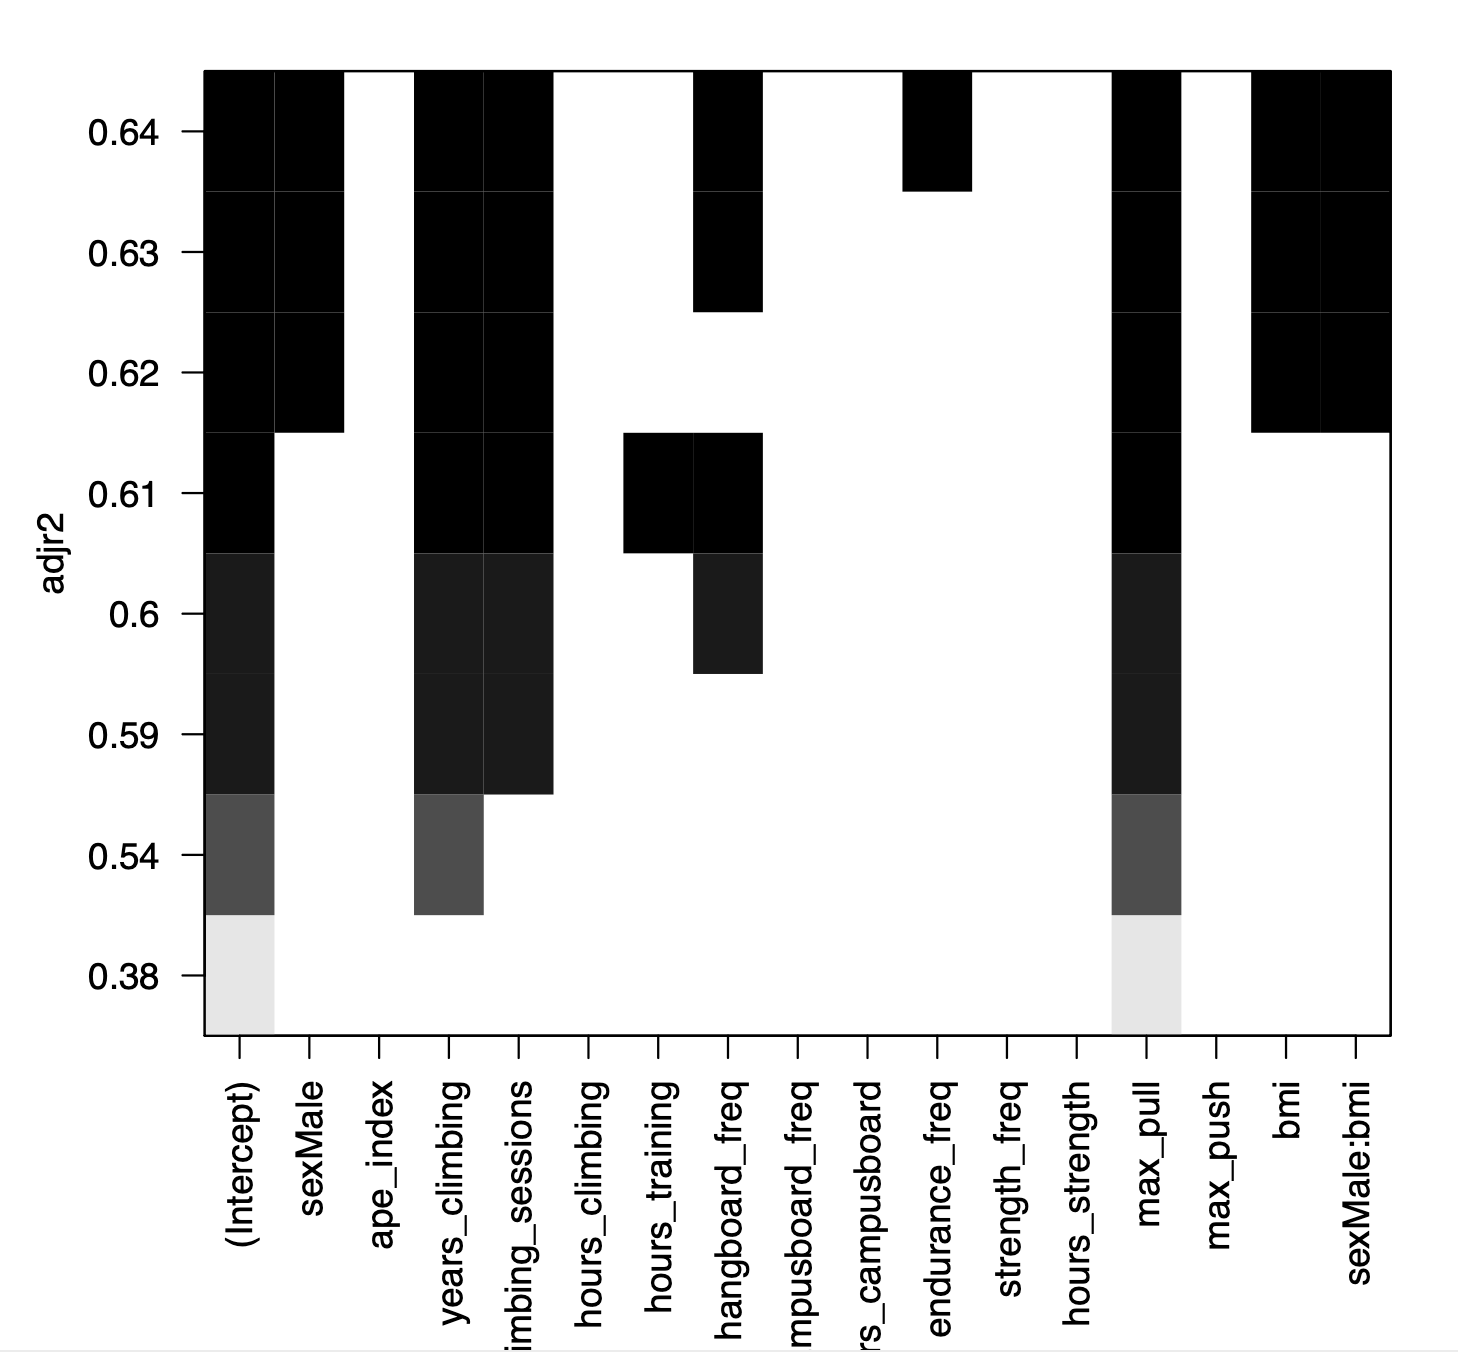
\includegraphics[width=0.5\textwidth]{rsq}
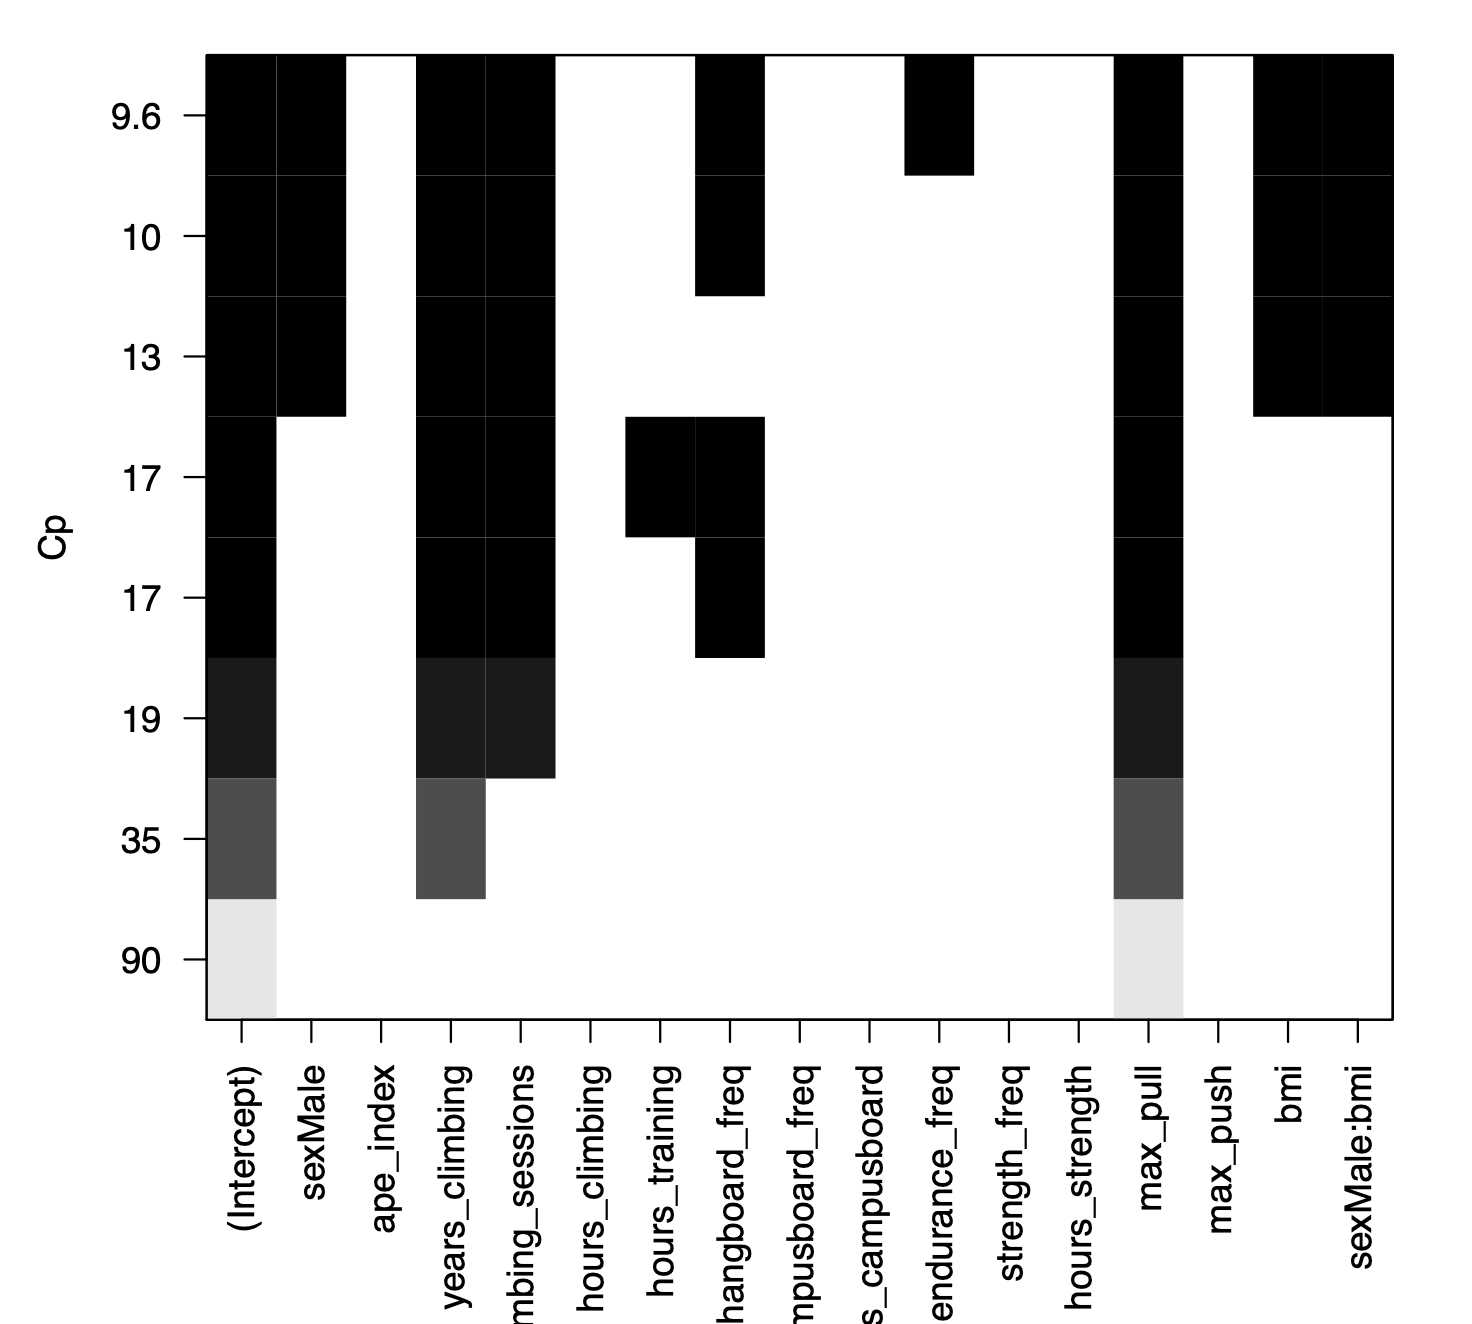
\includegraphics[width=0.5\textwidth]{cp}\\
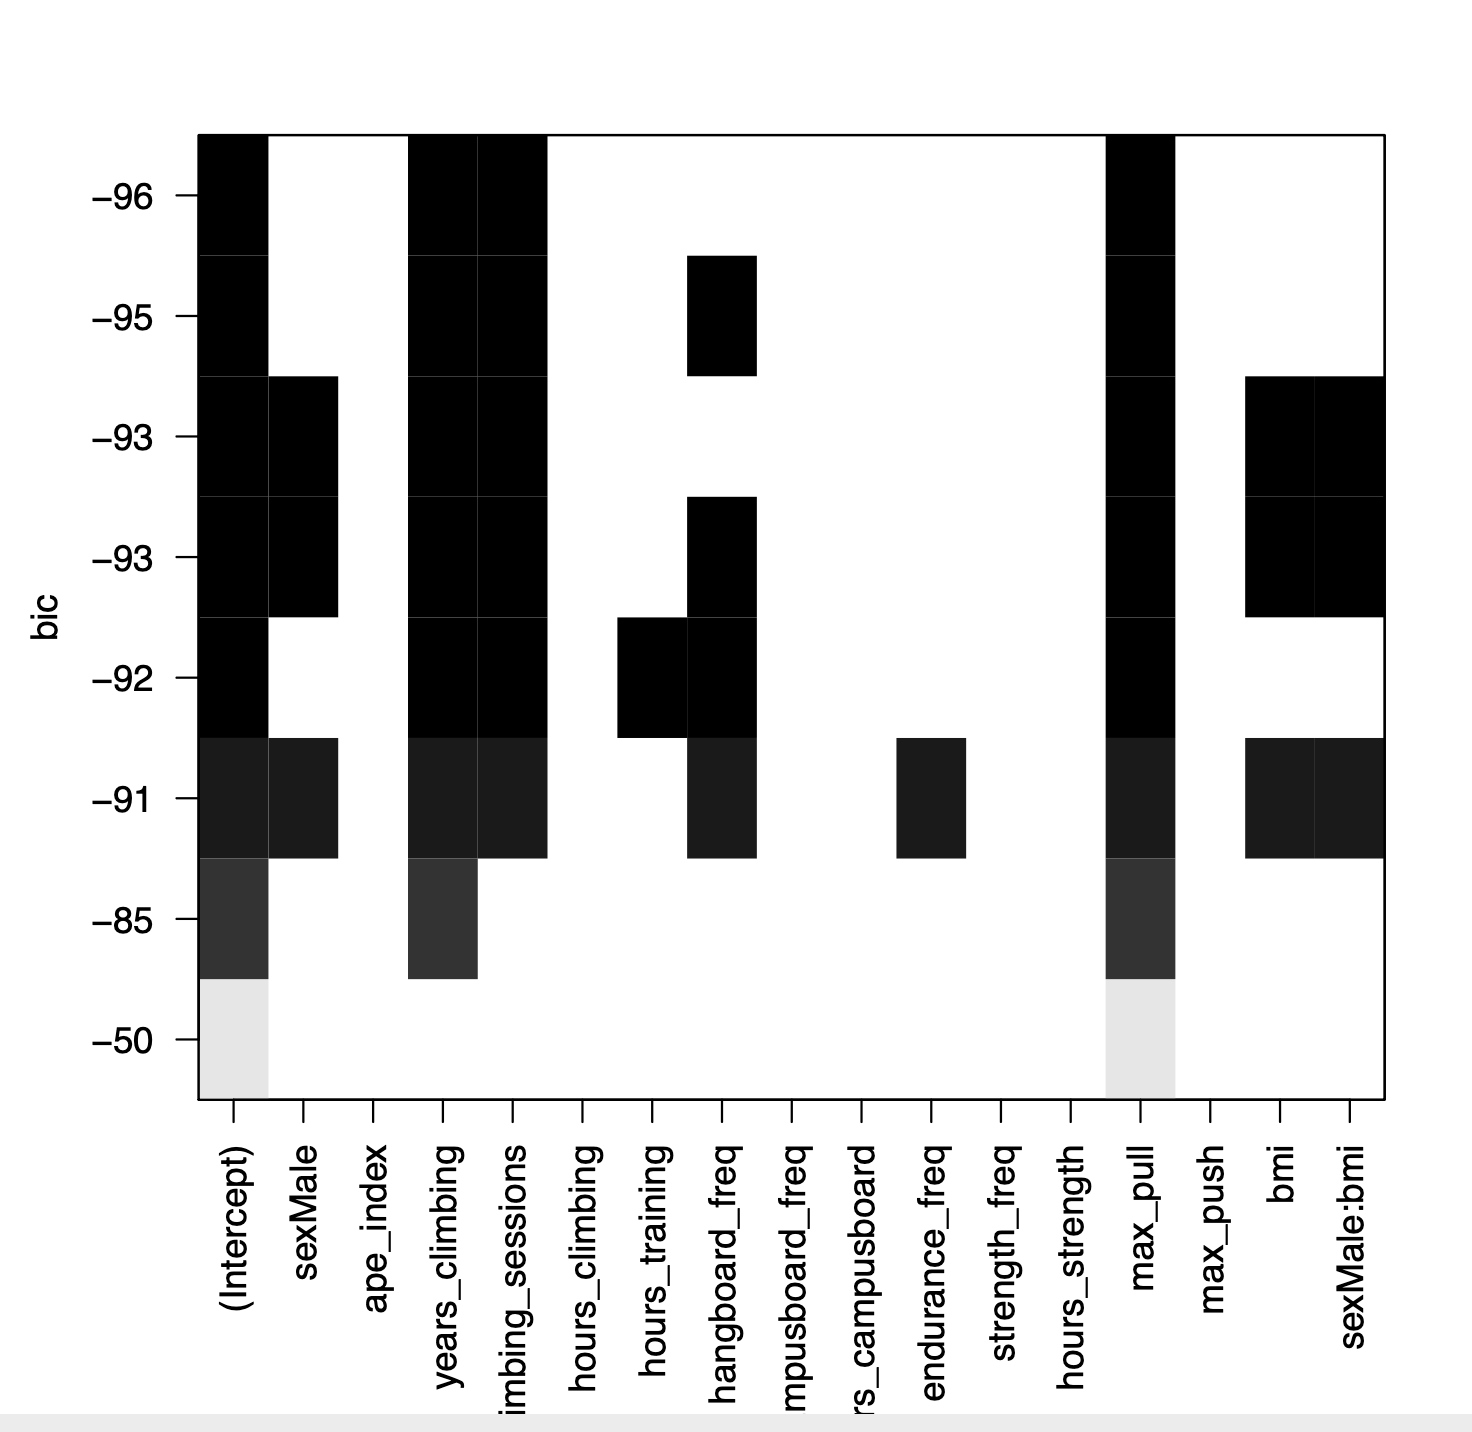
\includegraphics[width=0.6\textwidth]{bic}\\

Note that I also performed a forward selection, backward elimination, and a stepwise selection algorithm to the data. 
These criteria's didn't uncover anything novel - the exhaustive search was much more encompassing.


\newpage
{\bf\large Variable Selection Procedures Continued}\\
The utility of the model under investigation would be to make an unbiased prediction for training purposes, thus, we seek to maximize the adjusted $R^2$ value and minimize $\hat\sigma$.
Due to the various transformations of the best predictors, our interpretability of the model coefficients is limited.
Additionally, I believe we are missing some predictors that should be included in our model - assuming there even is a "true" regression model - so we will not try and make an inference on the individual coefficients.
After investigating the results that are suggested by the plots on the previous page, I settled on the following model:\\

\begin{center}
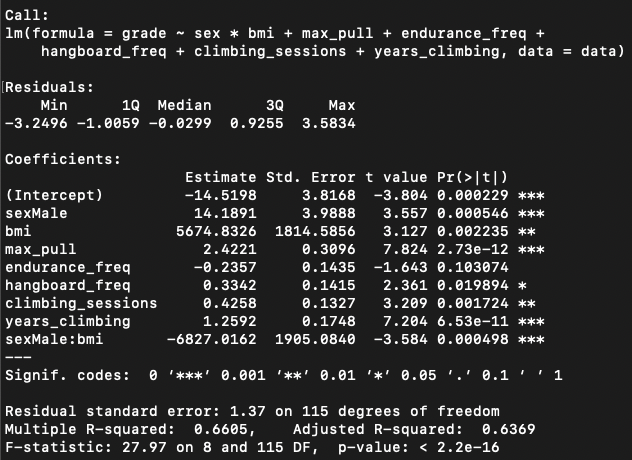
\includegraphics[width=0.7\textwidth]{summary}\\
\end{center}

Recall that a couple of the variables are transformed, so the actual linear model Rish formula is\\

\begin{center}
grade $\adj$ ln(years\_climbing + 1) + ln(max\_pull) + max\_push$^{-0.5}$ + sex + bmi + sex:bmi + endurance\_freq + hangboard\_freq + climbing\_sessions.\\
\end{center}




This model is appealing because it adequently meets our assumptions and has the smallest 
mallows $C_p$ value. Specifically, $C_p=9.6$ which is approximately equal to the number of columns in it's corresponding model matrix.
Though, it is slightly larger which may be an indication that our model is not taking into account a needed predictor.
That is, it may be an underfitted model.\\

\newpage
{\bf\large Final Model Assumption Diagnostics}\\
Next we take a look at our standard assumptions on this model.
The Shapiro test for normallity of the standardized residuals reports a p-value of $0.85$, which strongly supports our assumption that the residuals are normally distributed.
However, much stronger evidence is shown in the histogram and normal q-q plot.
Both of these plots can be found in Rplots.pdf and are omitted because they are great examples of plots generated from normally distributed residuals. 
The Breusch-Pagan test reports a p-value of $0.47$, which is evidence that our constant variance assumption of the residuals is not violated. 
The homoscedasticty assumption is strengthened by the lack of a funnel pattern in a plot of normal residuals verse the models fitted values.
This can also be concluded from the lack of an increasing or decreasing trend when we standardize the residuals to obtain the scale-location plot.\\
\begin{center}
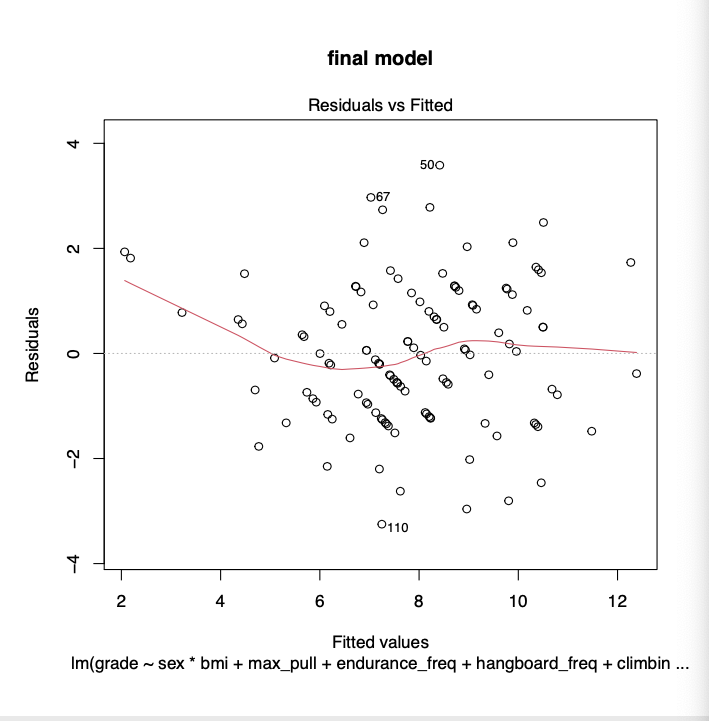
\includegraphics[width=0.55\textwidth]{resid1}\\
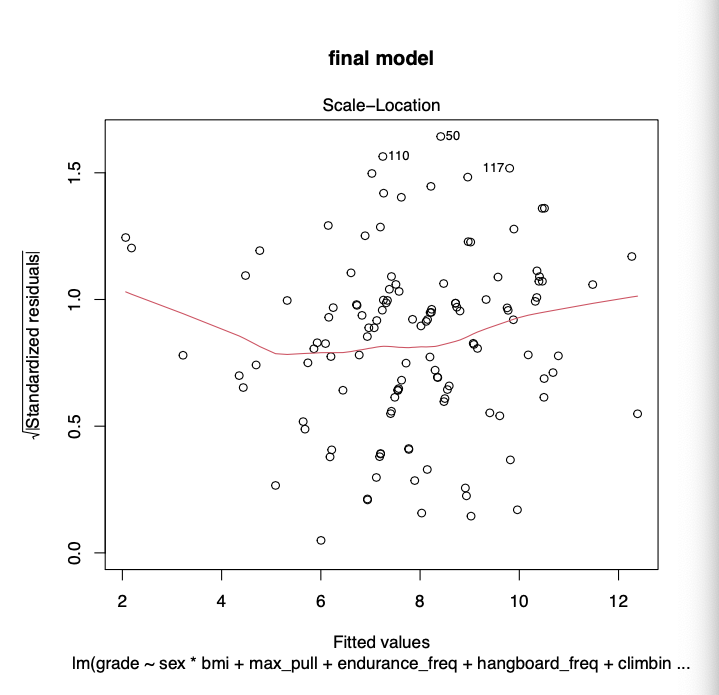
\includegraphics[width=0.55\textwidth]{scale}
\end{center}

\newpage
{\bf\large Final Model Assumption Diagnostics Continued}\\
Furthermore, when looking at both the plots on the previous page there is no obvious violation of our linearity assumption.
The next step is to look at our residual plots verse each predictor, where a linearity violation (or constant variance assumption) may become apparent.\\

\begin{center}
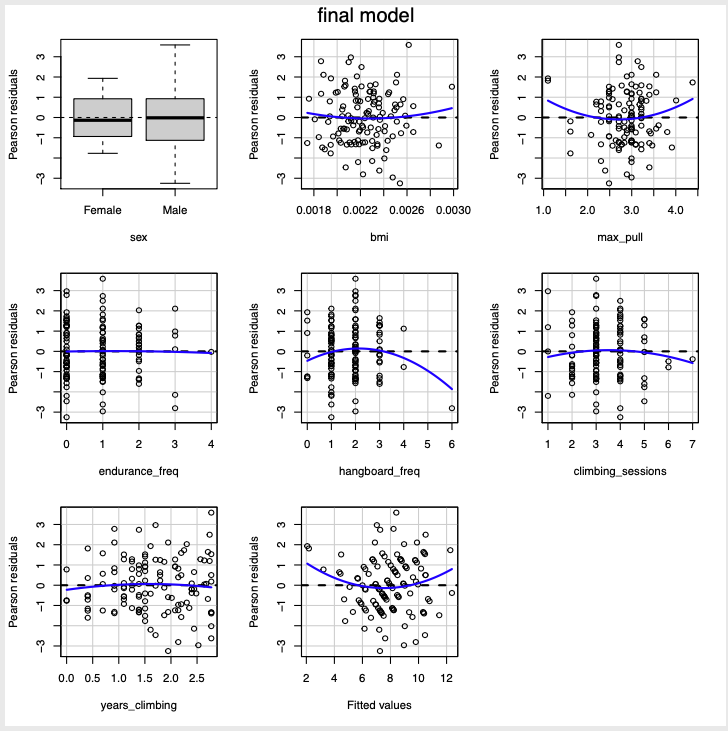
\includegraphics[width=0.56\textwidth]{resid3}
\end{center}

There is an outlier in the hangboard\_freq varible, but a transformation to address the problem is not warranted in my opinion.
The Tukey's test of additivity does not report a highly significant p-value to support the inclusion of any quadratic terms. Also, there is a potential violation of our constant variance assumption by the slight funneling in the years\_climbing plot - nothing we can really do.
Next note that there are no high-leverage/influential observationns in our data, as shown by the plot below.
\begin{center}
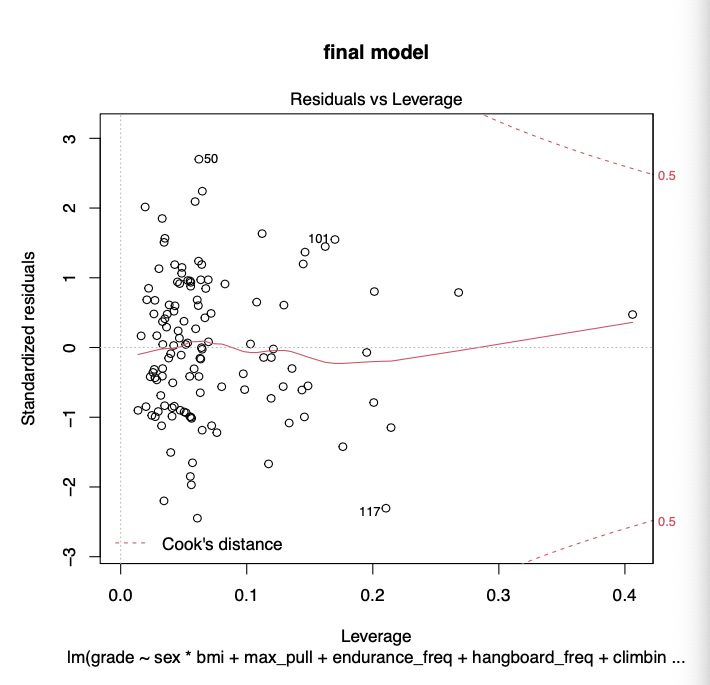
\includegraphics[width=0.5\textwidth]{leverage}
\end{center}

\newpage
{\bf\large Final Model Assumption Diagnostics Continued}\\
In conclusion, this model specification and consequent assumptions about the residuals are probably as good as we can get.
And recall that we didn't uncover a presence of collinearity earlier, so we safely assume that there is not a strong linear relationship between any of the predictor's in our final model matrix.
That is, (I believe) it is safe to assume that the conditioning of this least-squares problem is not of concern soley based upon my previous work. 




























\end{document}